%-----------------------------------------------------------------------------------------------------------------------------------------------%
%	The MIT License (MIT)
%
%	Copyright (c) 2021 Jitin Nair
%
%	Permission is hereby granted, free of charge, to any person obtaining a copy
%	of this software and associated documentation files (the "Software"), to deal
%	in the Software without restriction, including without limitation the rights
%	to use, copy, modify, merge, publish, distribute, sublicense, and/or sell
%	copies of the Software, and to permit persons to whom the Software is
%	furnished to do so, subject to the following conditions:
%	
%	THE SOFTWARE IS PROVIDED "AS IS", WITHOUT WARRANTY OF ANY KIND, EXPRESS OR
%	IMPLIED, INCLUDING BUT NOT LIMITED TO THE WARRANTIES OF MERCHANTABILITY,
%	FITNESS FOR A PARTICULAR PURPOSE AND NONINFRINGEMENT. IN NO EVENT SHALL THE
%	AUTHORS OR COPYRIGHT HOLDERS BE LIABLE FOR ANY CLAIM, DAMAGES OR OTHER
%	LIABILITY, WHETHER IN AN ACTION OF CONTRACT, TORT OR OTHERWISE, ARISING FROM,
%	OUT OF OR IN CONNECTION WITH THE SOFTWARE OR THE USE OR OTHER DEALINGS IN
%	THE SOFTWARE.
%	
%
%-----------------------------------------------------------------------------------------------------------------------------------------------%

%----------------------------------------------------------------------------------------
%	DOCUMENT DEFINITION
%----------------------------------------------------------------------------------------

% article class because we want to fully customize the page and not use a cv template
\documentclass[a4paper,12pt]{article}

%----------------------------------------------------------------------------------------
%	FONT
%----------------------------------------------------------------------------------------

% % fontspec allows you to use TTF/OTF fonts directly
% \usepackage{fontspec}
% \defaultfontfeatures{Ligatures=TeX}

% % modified for ShareLaTeX use
% \setmainfont[
% SmallCapsFont = Fontin-SmallCaps.otf,
% BoldFont = Fontin-Bold.otf,
% ItalicFont = Fontin-Italic.otf
% ]
% {Fontin.otf}

%----------------------------------------------------------------------------------------
%	PACKAGES
%----------------------------------------------------------------------------------------
\usepackage{url}
\usepackage{parskip} 	

%other packages for formatting
\RequirePackage{color}
\RequirePackage{graphicx}
\usepackage[usenames,dvipsnames]{xcolor}
\usepackage[scale=0.9]{geometry}
% \usepackage[a4paper,left=1cm,right=1cm,top=0.4cm,bottom=1.2cm]{geometry}

%tabularx environment
\usepackage{tabularx}

%for lists within experience section
\usepackage{enumitem}

% centered version of 'X' col. type
\newcolumntype{C}{>{\centering\arraybackslash}X} 

%to prevent spillover of tabular into next pages
\usepackage{supertabular}
\usepackage{tabularx}
\newlength{\fullcollw}
\setlength{\fullcollw}{0.47\textwidth}

%custom \section
\usepackage{titlesec}				
\usepackage{multicol}
\usepackage{multirow}

\usepackage{CJKutf8} % 核心包
\usepackage{tikz}
\usepackage{bm}
\usepackage{amssymb}

% ================= Profile Photo Parameters =================
\newcommand{\PhotoXShift}{-2.55cm}   % 整个头像：左右位置
\newcommand{\PhotoYShift}{-2.45cm}   % 整个头像：上下位置

\newcommand{\PhotoRadius}{1.4cm}    % 圆形头像半径
\newcommand{\PhotoImageWidth}{3.1cm} % 原图片缩放大小

\newcommand{\PhotoInnerXShift}{0cm}  % 图片在圆框内部左右移动
\newcommand{\PhotoInnerYShift}{-0.5cm}  % 图片在圆框内部上下移动

% 定义简写命令，写中文套 \cn{中文}
\newcommand{\cn}[1]{\begin{CJK}{UTF8}{gkai}#1\end{CJK}}

\usepackage[
    backend=biber,
    style=numeric,
    sorting=none
]{biblatex}

\addbibresource{citations.bib}

% Bibliography spacing
\setlength{\biblabelsep}{0.3em}
\setlength{\bibitemsep}{1em}

% Count bibliography items
\newcounter{publicationcount}
\AtEveryBibitem{\stepcounter{publicationcount}}

% Counter for patents
\newcounter{patentcount}

% Patent list: use the same layout as biblatex bibliography
\newenvironment{patentlist}
{%
    \begin{list}{}{%
        \setlength{\labelwidth}{\labelnumberwidth}%
        \setlength{\labelsep}{\biblabelsep}%
        \setlength{\leftmargin}{\labelwidth}%
        \addtolength{\leftmargin}{\labelsep}%
        \setlength{\itemindent}{0pt}%
        \setlength{\listparindent}{0pt}%
        \setlength{\parsep}{0pt}%
        \setlength{\itemsep}{\bibitemsep}%
        \setlength{\topsep}{0pt}%
    }%
}
{%
    \end{list}
}

\newcommand{\patent}[1]{%
    \stepcounter{patentcount}%
    \item[\mkbibbrackets{\number\numexpr
        \value{publicationcount}+\value{patentcount}\relax}]%
    #1%
}

\addbibresource{citations.bib}
\setlength{\biblabelsep}{0.3em}
\setlength{\bibitemsep}{0.3em}


%CV Sections inspired by: 
%http://stefano.italians.nl/archives/26
\titleformat{\section}{\Large\scshape\raggedright}{}{0em}{}[\titlerule]
\titlespacing{\section}{0pt}{7pt}{10pt}
% \titlespacing{\subsection}{0pt}{4pt}{6pt}

%for publications
% \usepackage[style=authoryear,sorting=ynt, maxbibnames=2]{biblatex}

%Setup hyperref package, and colours for links
\usepackage[unicode, draft=false]{hyperref}
\definecolor{linkcolour}{rgb}{0,0.2,0.6}
\hypersetup{colorlinks,breaklinks,urlcolor=linkcolour,linkcolor=linkcolour}
% \addbibresource{citations.bib}
% \setlength\bibitemsep{1em}

%for social icons
\usepackage{fontawesome5}

%debug page outer frames
%\usepackage{showframe}


% job listing environments
\newenvironment{jobshort}[2]
    {
    \begin{tabularx}{\linewidth}{@{}l X r@{}}
    \textbf{#1} & \hfill &  #2 \\[3.75pt]
    \end{tabularx}
    }
    {
    }

\newenvironment{joblong}[2]
    {
    \begin{tabularx}{\linewidth}{@{}l X r@{}}
    \textbf{#1} & \hfill &  #2 \\[3.75pt]
    \end{tabularx}
    \begin{minipage}[t]{\linewidth}
    \begin{itemize}[nosep,after=\strut, leftmargin=1em, itemsep=3pt,label=--]
    }
    {
    \end{itemize}
    \end{minipage}    
    }



%----------------------------------------------------------------------------------------
%	BEGIN DOCUMENT
%----------------------------------------------------------------------------------------
\begin{document}

% non-numbered pages
\pagestyle{empty} 

%----------------------------------------------------------------------------------------
%	TITLE
%----------------------------------------------------------------------------------------

% Profile photo -- overlay, does not affect centering of the header
% ================= Circular Profile Photo =================
\begin{tikzpicture}[remember picture,overlay]

    % Define center of profile photo
    \coordinate (photoCenter) at
    ([xshift=\PhotoXShift,yshift=\PhotoYShift]current page.north east);

    % Circular crop
    \begin{scope}
        \clip (photoCenter) circle (\PhotoRadius);

        \node at
        ([xshift=\PhotoInnerXShift,yshift=\PhotoInnerYShift]photoCenter)
        {
            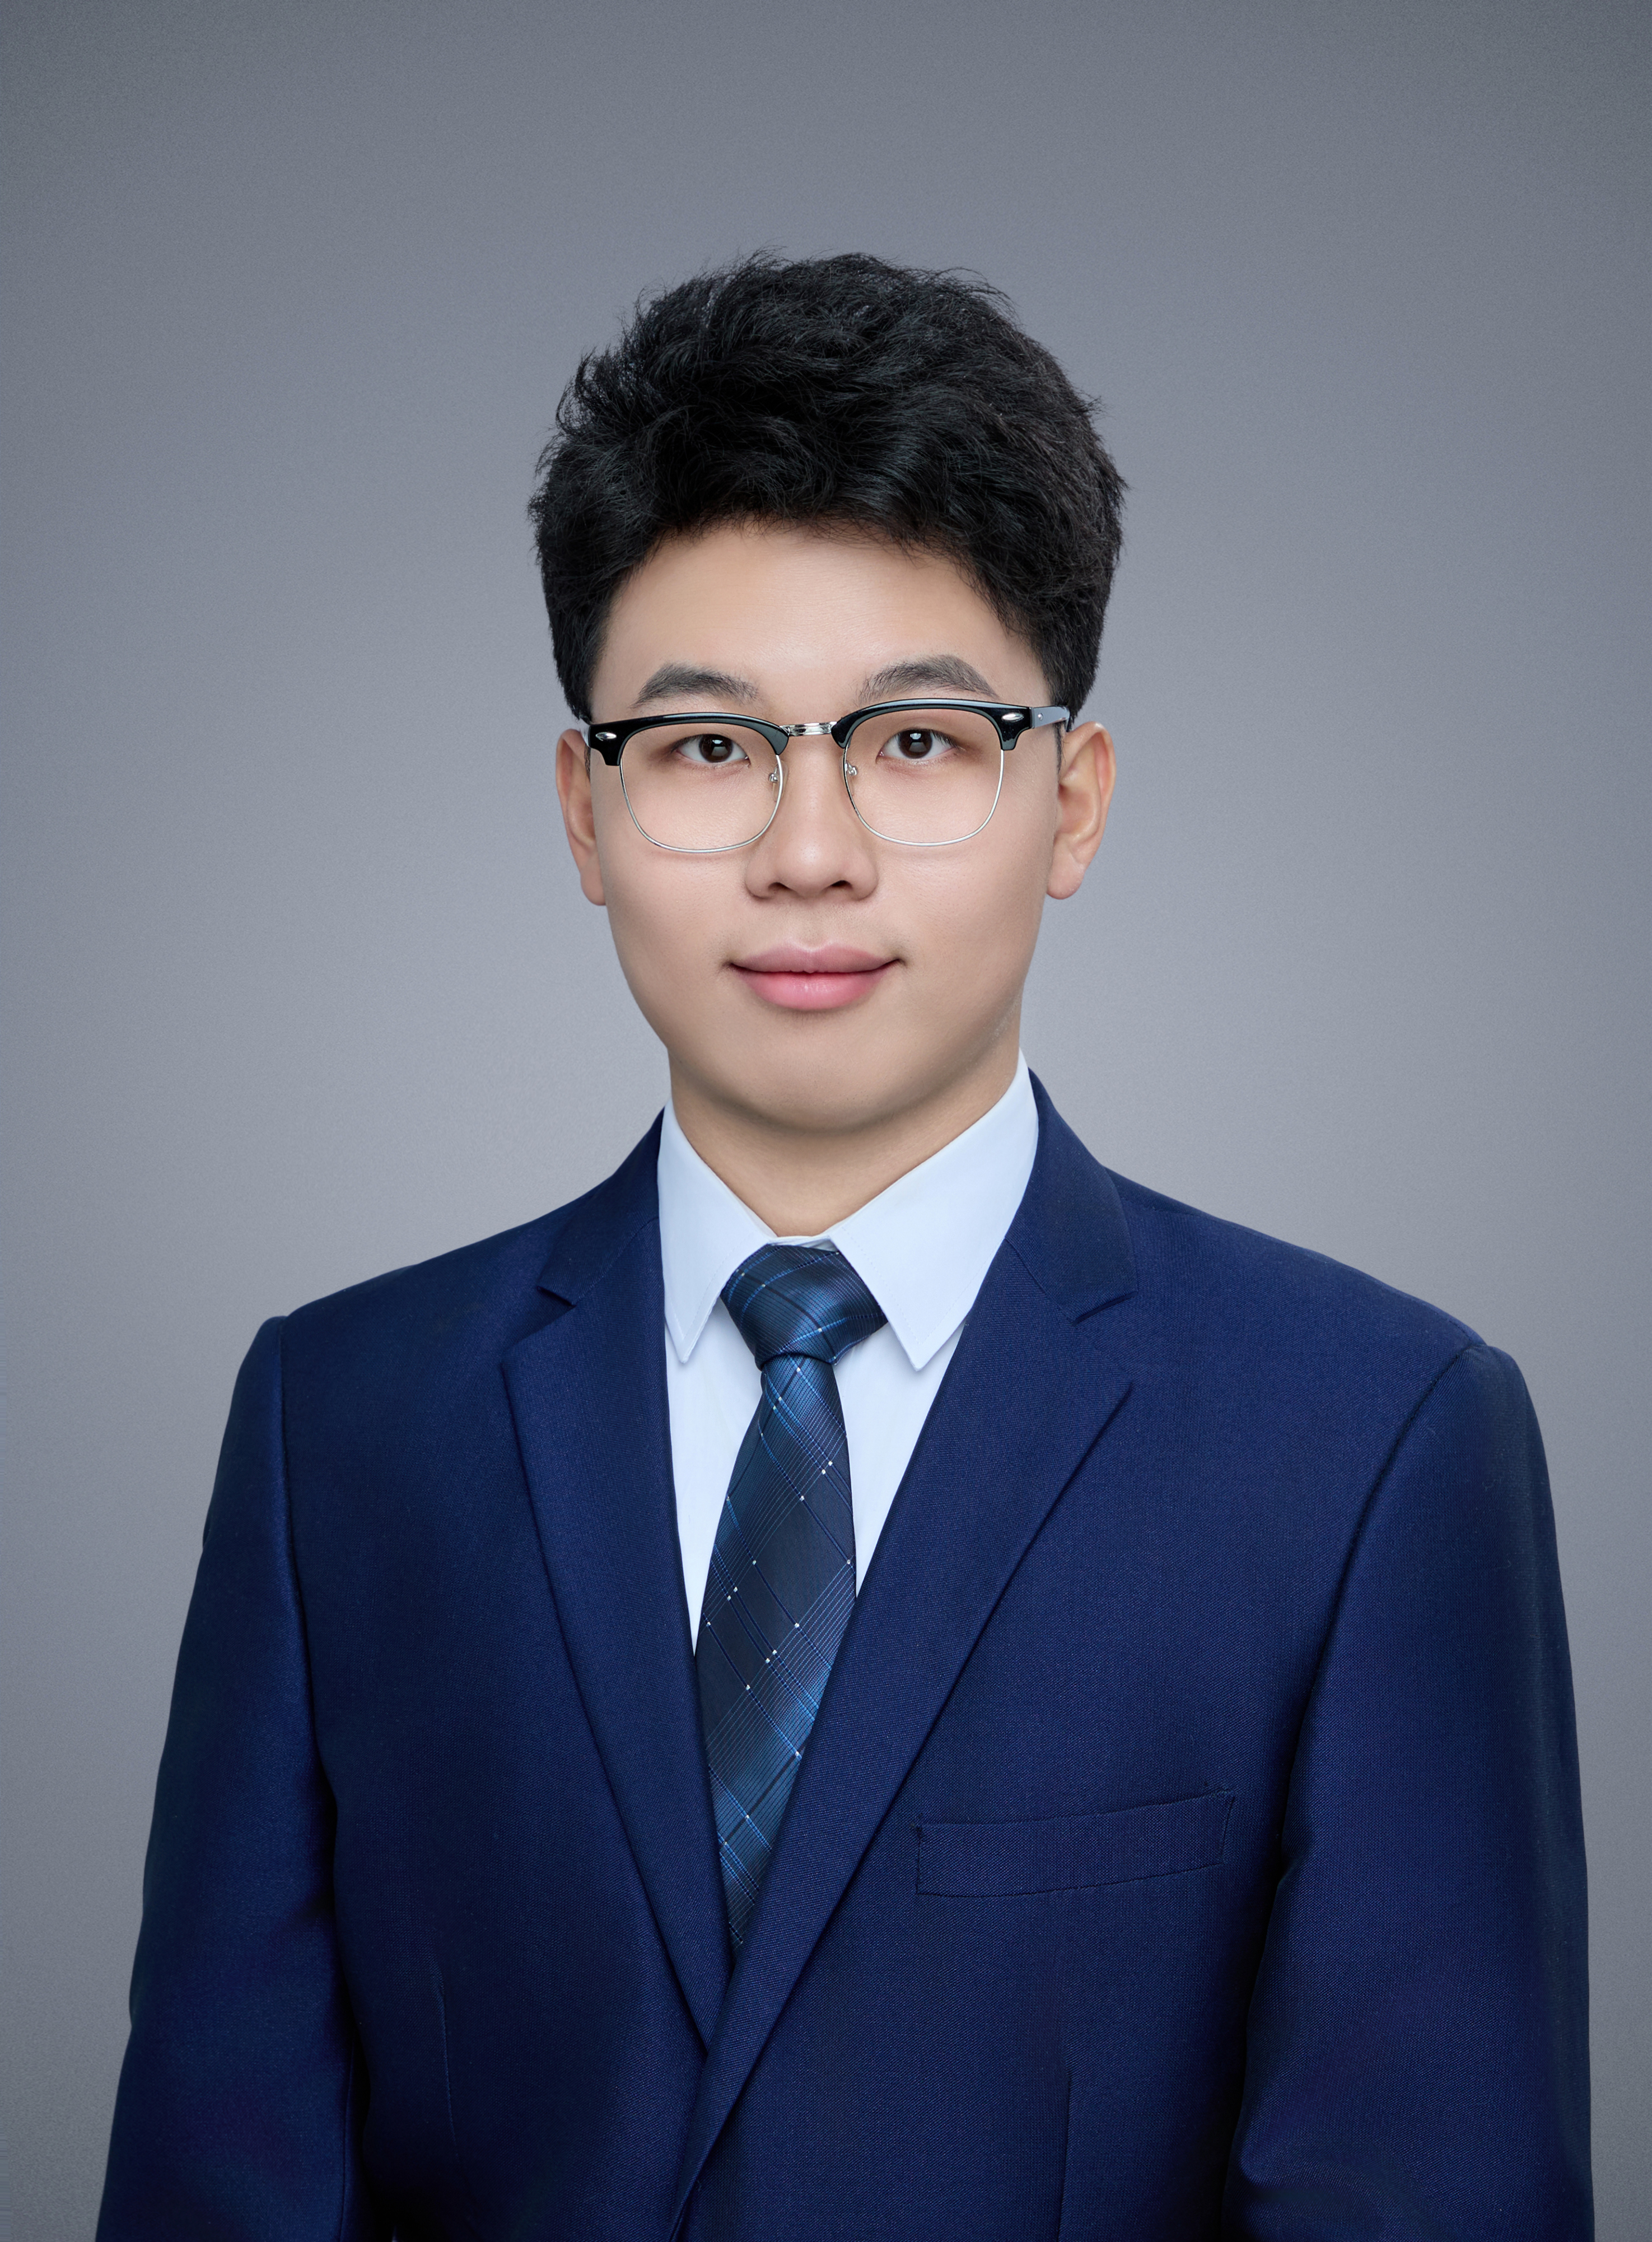
\includegraphics[
                width=\PhotoImageWidth
            ]{avatar.jpg}
        };
    \end{scope}

\end{tikzpicture}

\vspace*{-0.5cm}

\begin{tabularx}{\linewidth}{@{} C @{}}
\Huge{\bfseries Xiaoyu Yu (\cn{余骁宇})} \\[3pt]
\normalsize Mechanical Engineering, National University of Singapore \\[7.5pt]

\hspace*{-24mm}
\href{https://www.linkedin.com/in/shawyu666}{\raisebox{-0.05\height}\faLinkedin\ Linkedin} \ $|$ \ 
\href{https://scholar.google.com/citations?user=6xYnjXQAAAAJ\&hl=en\&inst=3212728378801010220}
{\raisebox{-0.05\height}\faUserGraduate\ Google Scholar} \ $|$ \
% \href{https://www.researchgate.net/}{\raisebox{-0.05\height}\faUserGraduate\ ResearchGate} \ $|$ \ 
\href{mailto:Shawyu@u.nus.edu}{\raisebox{-0.05\height}\faEnvelope \ Shawyu@u.nus.edu} \ $|$ \ 
\href{tel:+8615016867879}{\raisebox{-0.05\height}\faMobile \ +86 15016867879} \\
\end{tabularx}

%----------------------------------------------------------------------------------------
% EXPERIENCE SECTIONS
%----------------------------------------------------------------------------------------

%Interests/ Keywords/ Summary
\section{\textbf{Summary}}
Research interests include \textbf{quantitative modeling, machine learning, and data analytics}, \textbf{electrocatalytic materials and AI for Science}, and mathematical inverse problems, signal processing, and high-dimensional data reconstruction, with an interest in applications to quantitative finance.

%----------------------------------------------------------------------------------------
%	EDUCATION 
%----------------------------------------------------------------------------------------
% \section{\textbf{Education}}
% \begin{tabularx}{\linewidth}{@{}l X@{}}	
% Sep. 2023 -- Dec. 2025 & M.Sc Advancing Theory and Engineering at \textbf{Beihang University} 
% \hfill (Ranking 2/134, GPA: 3.78/4.0) \\
\section{\textbf{Education}}

\begin{itemize}[leftmargin=1.2em, itemsep=1pt, topsep=0pt]
    \item Ph.D. (Candidate) in Mechanical Engineering.,  \textbf{National University of Singapore} (NUS), Singapore
     \item M.Sc. in Advancing Theory and Engineering, \textbf{Beihang University} (BUAA), China 
    % \hfill (Ranking: 2/134, GPA: 3.78/4.0)
    \item B.Sc. (First) in Engineering, \textbf{Beihang University} (BUAA), China 
    % \hfill (Ranking: 5/89, GPA: 3.73/4.0)
    \item B.Sc. (Second) in Pure and Applied Mathematics, \textbf{Beihang University} (BUAA), China 
    % \hfill (Average Score: 91/100)
\end{itemize}

% Sep. 2019 -- Jun. 2023 & B.Sc Engineering in Aerospace (First Major) at \textbf{Beihang University} \hfill (Ranking 5/89, GPA: 3.73/4.0) \\ 

% Sep. 2020 -- Jun. 2023 & Bachelor of Science in Pure and Applied Mathematics (Second Major), School of Mathematical Sciences, \textbf{Beihang University} \hfill (Average Score: 91/100) \\
% \end{tabularx}




%Projects
\section{\textbf{Projects}}

\begin{tabularx}{\linewidth}{ @{}l r@{} }
\textbf{Mathematical Inverse Modeling and Multichannel Sensor Data Analysis}\\
% \\ Project Student Leader \\[3.75pt]
\multicolumn{2}{@{}X@{}}{
\begin{itemize}[leftmargin=*, label=—]
    \item Developed acoustic-scattering-based inverse methods to recover dynamic gas--liquid interface information from sensor measurements;
    \item Independently implemented signal inversion algorithms and custom data-processing software;
    \item Designed a synchronized multichannel ultrasonic measurement system, achieving millimeter-level bubble measurement accuracy in a cryogenic liquid-nitrogen environment (77 K).
\end{itemize}
} \\
\end{tabularx}

% \vspace*{0.2cm}
\begin{tabularx}{\linewidth}{ @{}l r@{} }
\textbf{Machine Learning for High-Dimensional Data Reconstruction} & \\
%& \hfill Project Student Leader \\[3.75pt]

\multicolumn{2}{@{}X@{}}{
\begin{itemize}[leftmargin=*, label=—, itemsep=0pt, labelsep=4pt]
    \item Developed a diffusion-model-based inversion framework using U-Net \& EDM, outperforming conventional neural networks with average reconstruction error below 2\%.
    \item Constructed a numerical dataset covering 416 operating conditions using elliptic PDE meshes for model development and evaluation.
    \item Evaluated reconstruction quality using structural similarity (SSIM) and quantitative error metrics, achieving 0.327\% relative error in transient-field reconstruction using DDIM sampling.
\end{itemize}
}  \\
\end{tabularx}

\begin{tabularx}{\linewidth}{ @{}l r@{} }
\textbf{Pt-Based Electrocatalyst Engineering for AOR} & \\
%& \hfill Project Student Leader \\[3.75pt]
\multicolumn{2}{@{}X@{}}{
\begin{itemize}[leftmargin=*, label=—, itemsep=0pt, labelsep=4pt]
    \item Designed and synthesized Pt/NiO-based catalysts by tuning Pt loading, substrates, and thermal treatment to investigate Pt-site configurations and metal--support interactions.
    \item Integrated CV, LSV, EIS, Tafel, and Raman analyses to assess AOR activity, charge-transfer kinetics, and potential structure--activity relationships associated with surface reconstruction.
\end{itemize}
}  \\
\end{tabularx}

\begin{tabularx}{\linewidth}{ @{}l r@{} }
\textbf{Quantitative Imaging and Experimental Data Analysis} & \\
%& \hfill Project Student Leader \\[3.75pt]
\multicolumn{2}{@{}X@{}}{
\begin{itemize}[leftmargin=*, label=—, itemsep=0pt, labelsep=4pt]
   \item  Developed high-speed PIV and 2D3C stereoscopic PIV platforms for quantitative flow-field reconstruction and nanoparticle tracking under extreme conditions (6 MPa, 100–600 m/s).

   \item  Applied high-speed imaging, laser interferometry, and subpixel edge detection to extract high-resolution spatial and temporal measurements of transient physical processes.

    \item Performed quantitative image and experimental data analysis to characterize particle trajectories, flow dynamics, and small-scale structural vibrations.
    
\end{itemize}
}  \\
\end{tabularx}



%----------------------------------------------------------------------------------------
%	PUBLICATIONS s
%----------------------------------------------------------------------------------------
\section{\textbf{Publications \& Patents}}
% \subsection{\textbf{Journal \& Conference Papers} (Selected)}
% \subsection*{\textgreater\ \textbf{Journal \& Conference Papers} (Selected)}
% \subsection*{\(\bm{>}\)\ \textbf{Journal \& Conference Papers} (Selected)}
\subsection*{\(\triangleright\)\  \textbf{Journal \& Conference Papers} (Selected)}

\begin{refsection}[citations.bib]
\nocite{*}
\printbibliography[
    heading=none,
    sorting=none
]
\end{refsection}


% [1] Xiaoyu Yu, Xiaokang Liu, Jingxuan Li et al. Impact of vibrating combustion chamber wall on flame thermoacoustic dynamics[J]. Physics of Fluids, 2025. (SCI Q1)

% [2] Xiaoyu Yu, Xiaokang Liu, Jingxuan Li, et al. Theoretical study on intrinsic thermo-acoustic mode in long flame combustion chamber[C]. China National Symposium on Combustion, China, 2024.

% [3] Xiaoyu Yu, Xiaokang Liu, Jingxuan Li, et al. The Influence of Lateral Offset of Laminar Premixed Flames on Thermoacoustic Instability of Burners[C]. The International Symposium On Multiscale Simulations Of Thermophysics, China, 2024.

% [4] Xiaokang Liu, Xiaolin Xiang, Xiaoyu Yu, et al. On the two approaches for the combustion instability predictions in a long-flame combustor[J]. Acta Astronautica, 2024. (SCI Q1)

% [5] Wuzhou Qin, Xiaoyu Yu, Jingxuan Li et al. Efficient Inverse Reconstruction of Internal Flow Fields in Rocket Engine Combustion Chambers Based on Diffusion Models[J]. Physics of Fluids, 2025. (SCI Q1)

% [6] Xiaoyu Yu, Jingxuan Li et al. Study on the mechanism of boundary vibration on flame fluid-thermal coupling[J]. Combustion and Flame, 2025. (Submitted, SCI Q1)

% [7] Xiaokang Liu, Xiaoyu Yu, Xudong Yu, et al; Measurement of jet gas–liquid interface fluctuations based on ultrasonic scattering[J]. Physics of Fluids, 2024; V36(1): 013333.(Featured Article SCI Q1)

% [8] Xiaokang Liu, Xiaoyu Yu, Jingxuan Li, et al. Ultrasonic scattering measurements of jet gas-liquid interface fluctuations in confined spaces[J]. Physics of Fluids, 2025; V37(2): 023306. (SCI Q1)

% [9] Jiangchang Chen, Xiaokang Liu, Xiaoyu Yu, Jingxuan Li et al. Ultrasonic Three Dimensional Reconstruction and Measurement Technology for Complex Propellant Free Surfaces[J]. Physics of Fluids, 2025,37(12). (SCI Q1)

% [10] Xiaokang Liu, Jingxuan Li, Xudong Yu, Xiaoyu Yu, et al. Measurement of jet gas-liquid interfaces in confined spaces based on ultrasonic scattering. 30th International Congress on Sound and Vibration, 2024. (EI)
\vspace*{-0.3cm}
\subsection*{\(\triangleright\)\ \textbf{Chinese Invention Patents} (Selected)}
%
% \subsection{\textbf{Chinese Invention Patents}}

\begin{patentlist}

\patent{Jingxuan Li, Xiaoyu Yu, et al. Measurement method for liquid bubble content in the test tank and measurement system for liquid bubble content in the test tank: 202410948864X [P] 2024.07.16}

% \patent{Jingxuan Li, Xiaoyu Yu, et al. Method for simulating bubble behavior in liquid under microgravity conditions in space on the ground: 2024109488616 [P] 2024.07.16}

\patent{Jingxuan Li, Xiaoyu Yu, et al. Adjustable flow solid nanoparticle generator: 2024102667367 [P] 2024.03.08}

% \patent{Jingxuan Li, Xiaoyu Yu, et al. Liquid level shape detection system in storage tank: 2024109488620 [P] 2024.07.16}

\patent{Jingxuan Li, Xiaoyu Yu, et al. A measurement method and device for gas-liquid interface of liquid jet in a closed environment: 202510096916X [P] 2025.01.22}

\end{patentlist}
% [11] Jingxuan Li, Xiaoyu Yu, et al. Measurement method for liquid bubble content in the test tank and measurement system for liquid bubble content in the test tank: 202410948864X [P] 2024.07.16

% [12] Jingxuan Li, Xiaoyu Yu, et al. Method for simulating bubble behavior in liquid under microgravity conditions in space on the ground: 2024109488616 [P] 2024.07.16

% [13] Jingxuan Li, Xiaoyu Yu, et al. Adjustable flow solid nanoparticle generator: 2024102667367 [P] 2024.03.08

% [14] Jingxuan Li, Xiaoyu Yu, et al. Liquid level shape detection system in storage tank: 2024109488620 [P] 2024.07.16

% [15] Jingxuan Li, Xiaoyu Yu, et al. A measurement method and device for gas-liquid interface of liquid jet in a closed environment: 202510096916X [P] 2025.01.22








%Experience
\section{\textbf{Work Experience}}

\begin{joblong}{Student Counselor, Beihang University Student Affairs Office}{}
% {Mar. 2021 -- Jul. 2025}
\item Responsible for daily office conference arrangement, administrative management and official document drafting work
\item Organized large-scale campus events, award ceremonies and freshman military training activities
\end{joblong}

\begin{jobshort}{Chairman, Graduate Student Union of the School of Astronautics}{}
Conducted comprehensive management and coordination of all functional departments; maintained communication and joint research with institutes and technical units.
\end{jobshort}

\begin{jobshort}{COVID-19 Campus Isolation Area Volunteer Leader}{}
Served as person-in-charge of campus isolation zone during pandemic prevention and control period.
\end{jobshort}


%----------------------------------------------------------------------------------------
%	SKILLS
%----------------------------------------------------------------------------------------
\section{\textbf{Skills, Honors \& Scholarships}}
\begin{tabularx}{\linewidth}{@{}l X@{}}
\textbf{Programming:} & Matlab, LabView, Fortran, C, C++, Python, JavaScript, Origin, Chat-GPT \\
\textbf{Software:} & AutoCAD Professional Qualification, SolidWorks Professional Qualification, MS Office Level 2 (National Computer Rank Examination)\\
\textbf{Languages:} & IELTS 6.5, CET-6 565 (Top 15\% nationwide), Mandarin (Native), Cantonese (Native)\\
\end{tabularx}

\vspace{6pt}
\textbf{Selected Scholarships:} National Scholarship (2025); BUAA Shenyuan Top Scholarship, CATIC Top-class Scholarship, Multiple First-Class Academic Scholarships; Mathematics \& Physics Competition Top Scholarship; Freshman Scholarship.

\vspace{6pt}
\textbf{Selected Honors:} National University Student Mathematics Competition First Prize (2021,2022); National Undergraduate Graduation Design Competition Second Prize (2023); BUAA Shenyuan Gold Medal (Top 10 students annually, 2025); Outstanding Graduate; Excellent Student Cadre

\vspace{6pt}
\textbf{Extracurricular Sports:} Badminton Team Champion; Football Runner-up (twice); Basketball Team Champion; Table Tennis, Vocal music.


% \vfill
% \center{\footnotesize Last updated: \today}

\end{document}
